\documentclass{article}

\usepackage{amsmath}
\usepackage{graphicx}

\newcommand{\rr}{\mathbf{r}}

\begin{document}

{\bf Quiz \#11; Tuesday, date: 04/10/2018}

{\bf MATH 53 Multivariable Calculus with Stankova}

{\bf Section \#114; time: 2 -- 3:30 pm}

{\bf GSI name: Kenneth Hung}

{\bf Student name: SOLUTIONS}

\vspace*{0.25in}

\begin{enumerate}
\item Find the gradient vector field $\nabla f$ of $f$ and sketch it.
\[
f(x, y) = x(x+y)
\]

{\em Solution.} We take the gradient directly.
\[
\nabla f(x, y) = \langle 2x + y, x \rangle
\]
To sketch it, we start by checking the vector field on the axis. On the $x$-axis, the vector is $\langle 2x, x \rangle$. So they are all parallel but with different magnitude / direction. On the $y$-axis, the vector is $y, 0$. Inspired by this, we can also observe that along the line $2x + y = 0$, the gradient vector is always vertical. Putting all these information in the sketch gives
\begin{center}
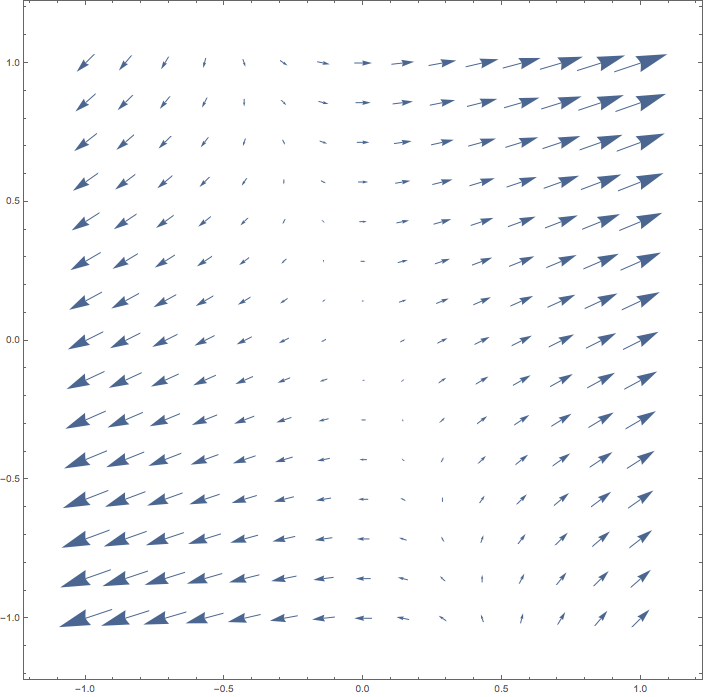
\includegraphics[width=0.6\textwidth]{quiz11dis114solpic}
\end{center}

\item {\em True / False?} $\mathbf{F}(x, y) = \langle x^2, y^2 \rangle$ is a conservative vector field.

{\em Solution.} {\bf True.} It can be written as the gradient of the function $\frac{1}{3} x^3 + \frac{1}{3} y^3$.

\item {\em True / False?} Suppose $f$ is a scalar function and $\nabla f$ is a force field. The work done by this force field along any one level curve of $f$ maybe nonzero.

{\em Solution.} {\bf False.} The gradient is always perpendicular to the level curves. So the tangent along any level curve is perpendicular to the force field at all times. Since $\mathbf{F} \cdot \mathbf{T} = 0$, there is no work done.

\end{enumerate}

\end{document}